\documentclass{iopconfser}

\usepackage{float}
\usepackage{graphicx}
\usepackage{subcaption}
\usepackage[automake]{glossaries-extra}
\usepackage{ragged2e}
\usepackage[export]{adjustbox}
\usepackage{mathtools}
\usepackage{setspace}
\onehalfspacing
% \makeglossaries

\setabbreviationstyle[acronym]{long-postshort-user}
\glssetcategoryattribute{acronym}{nohyperfirst}{true}
\setabbreviationstyle{short-nolong}
\makeglossaries

% --------------------
% ---- Glossaries ----
% --------------------
\newglossaryentry{asyncio}{name=Asyncio, description={A Python library for asynchronous code.}}
\newglossaryentry{stim}{name=STIM300, description={A MEMS-based \gls{imu}}}
\newglossaryentry{f9p}{name=F9P, description={A Global Navigation Satellite System (GNSS) receiver manufactured by u-blox.}}

% --------------------
% ----- Acronyms -----
% --------------------
\newacronym{asv}{ASV}{Autonomous Surface Vehicle}
\newacronym{dolp}{DoLP}{Degree of Linear Polarization}
\newacronym{aolp}{AoLP}{Angle of Linear Polarization}
\newacronym{sitaw}{SITAW}{Situational Awareness}
\newacronym{poe}{PoE}{Power over Ethernet}
\newacronym{pps}{PPS}{Pulse Per Second}
\newacronym{cpfa}{CPFA}{Color-Polarization Filter Array}
\newacronym{utc}{UTC}{Coordinated Universal Time}
\newacronym{imu}{IMU}{Inertial Measurement Unit}
\newacronym{tov}{TOV}{Time of Validity}
\newacronym{tm2}{TM2}{Time mark data}
\newacronym{gnss}{GNSS}{Global Navigation Satellite System}
\newacronym{ptp}{PTP}{Precision Time Protocol}

% \glsaddall
% \makenoidxglossaries

% \glsunset{cpu}
\glsunset{gnss}
\glsunset{imu}
\glsunset{tm2}
\glsunset{utc}

% --------------------
% ----- Shortcuts ----
% --------------------


\addbibresource{mylib.bib}


\begin{document} 

\title{AI Powered Mini Ferries, the Future of Urban Transportation or Just a Hype?}

\section*{<<MilliAmpere 2>>, the new research ship from NTNU, gives us sneak peek of how bridges might become obsolete in future cities.}

\begin{figure}[H]
    \centering
    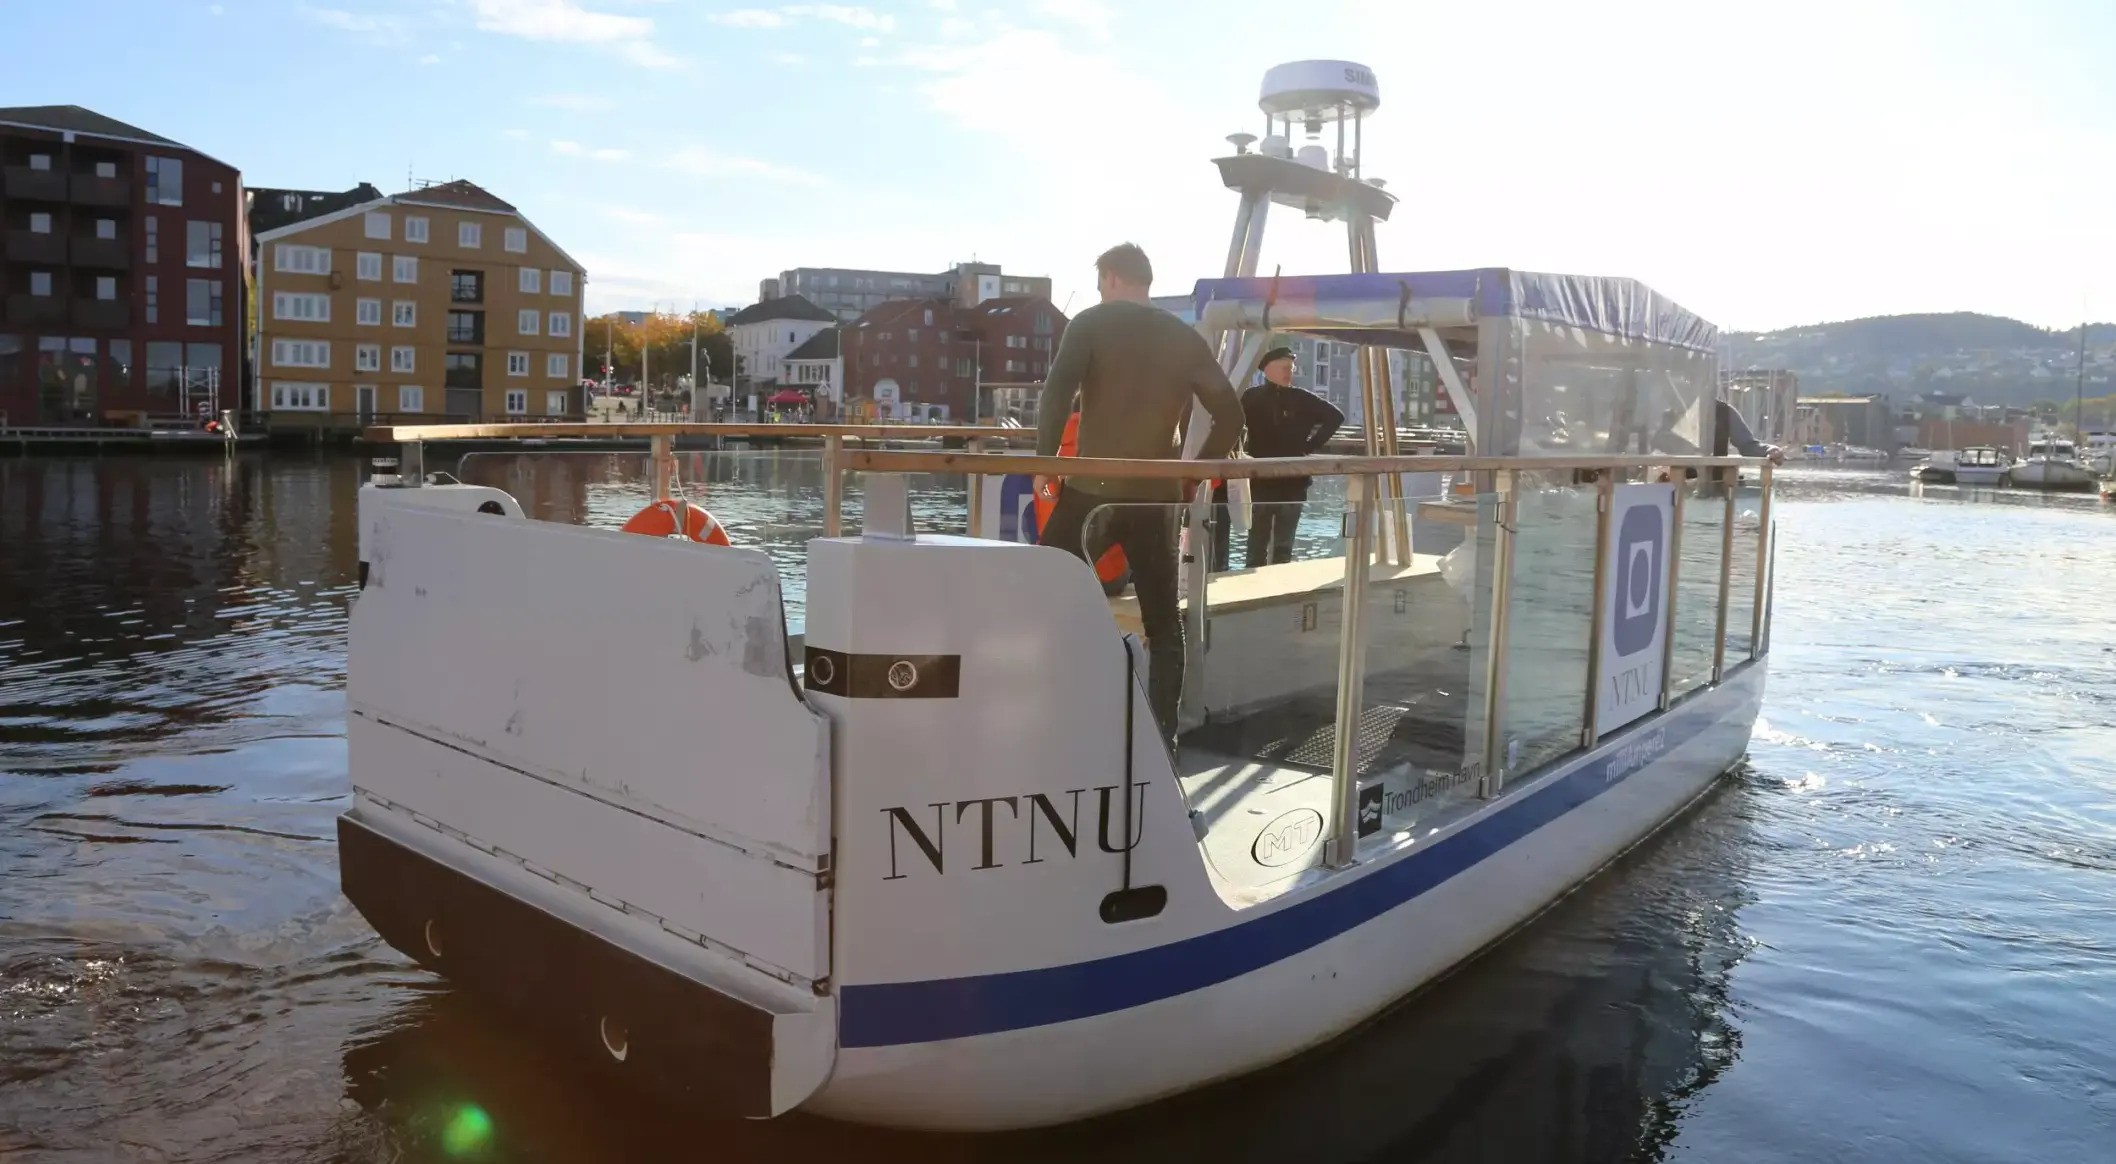
\includegraphics[width=\textwidth]{figures/milliampere.jpg}
    \caption{MilliAmpere 2 driving autonomously in Trondheim harbour \cite{hauglandDetSomHar2022}.}
\end{figure}

\section*{Artificial Intelligence in Autonomous Vehicles}
The word AI gets thrown around a lot these days, so lets clarify what we mean by AI in this context.
As an experienced driver you generally don't have to think a lot when driving a car.
You just have to stay in you lane, keep a safe distance to other vehicles and follow the speed limit.
Most of these things can already be done by a modern car as well, with adaptive cruise control and lane keeping assist.
These things are not considered as AI but rather as advanced automation, where a human has defined the rules for what to do.

When something unexpected happens however, you as a driver have to react quickly and make the right decision.
This ability to react to a new and unexpected situations is what is currently missing in autonomous vehicles and is what we refer to as AI when talking about autonomous vehicles.
The problem can be broken into three parts; 1) realizing that something unexpected is happening 2) understanding what that is 3) deciding what to do about it.


\section*{Ferries VS Cars}
Autonomous cars is something that appears to always just be a couple of years away, yet never seems to arrive.
Billions of dollars have been invested into their development but the technology is still not ready for widespread use. 
Why is the development of autonomous ferries any different?

When we start to deploy autonomous vehicles, ehther cars or ferries, there will be a transition period where a human operator is monitoring the vehicle and can take control if needed. 
For autonomous cars, the operator needs to be behind the wheel at all times to be able to react quikly enough and avoid accidents.
Ferries however are a different story.
They move significantly slower than cars, have better overview, cannot cause congestions and do not have to deal with pedestrians in the same way as road vehicles.
An autonomous ferry therefore really only needs to be able to detect that something unexpected is happening, stand still and alert a remote operator and wait for them to take control.
Being stuck on a ferry waiting for a remote operator to take control might be annoying, but it is not dangerous.
This makes the transition to fully autonomous ferries much more gradual and less risky than for cars.





% \printglossary
\printbibliography


\end{document}